\documentclass[11pt]{article}
\usepackage[textwidth=18.0cm, textheight=23.0cm, top=2.0cm]{geometry}
\usepackage{pst-all}
\usepackage{amssymb}
\usepackage{tikz}
\usepackage{underscore}\begin{document}
\pagestyle{empty}


ClassName: \underline{\textbf{Class_07.2bp-29}}
\par
BinSize: \underline{\textbf{100 × 100}}
\par
ReduceSize: \underline{\textbf{100 × 100}}
\par
TypeNum: \underline{\textbf{60}}
\par
Num: \underline{\textbf{60}}
\par
OutS: \underline{\textbf{190000}}
\par
InS: \underline{\textbf{162038}}
\par
Rate: \underline{\textbf{0.853}}
\par
UB: \underline{\textbf{19}}
\par
LB0: \underline{\textbf{18}}
\par
LB: \underline{\textbf{18}}
\par
LBWithCut: \underline{\textbf{19}}
\par
NodeCut: \underline{\textbf{1}}
\par
ExtendedNodeCnt: \underline{\textbf{1}}
\par
GenNodeCnt: \underline{\textbf{1}}
\par
PrimalNode: \underline{\textbf{0}}
\par
ColumnCount: \underline{\textbf{180}}
\par
TotalCutCount: \underline{\textbf{33}}
\par
RootCutCount: \underline{\textbf{33}}
\par
LPSolverCnt: \underline{\textbf{163}}
\par
PricingSolverCnt: \underline{\textbf{163}}
\par
BranchAndBoundNum: \underline{\textbf{1}}
\par
isOpt: \underline{\textbf{true}}
\par
TimeOnInitSolution: \underline{\textbf{120.010 s}}
\par
TimeOnPrimal: \underline{\textbf{0.000 s}}
\par
TimeOnPricing: \underline{\textbf{19.038 s}}
\par
TimeOnRmp: \underline{\textbf{0.149 s}}
\par
TotalTime: \underline{\textbf{139.401 s}}
\par
\newpage



\begin{tikzpicture}[shorten >=1pt,scale=1.0,every node/.style={scale=1.0},->]
\tikzstyle{vertex}=[circle,fill=black!25,minimum size=14pt,inner sep=0pt]
\filldraw[fill=gray!40!white, draw=black] (0,0) rectangle (15.0,15.0);
\foreach \name/\x/\y/\w/\h in {98x88/0.0/0.0/14.7/13.2}
\filldraw[fill=white!40!white, draw=black] (\x,\y) rectangle node[draw] (\name) {\name} ++(\w,\h);
\end{tikzpicture}


w =98 , h =88 , x =0 , y =0 , v =8624
\par
\newpage


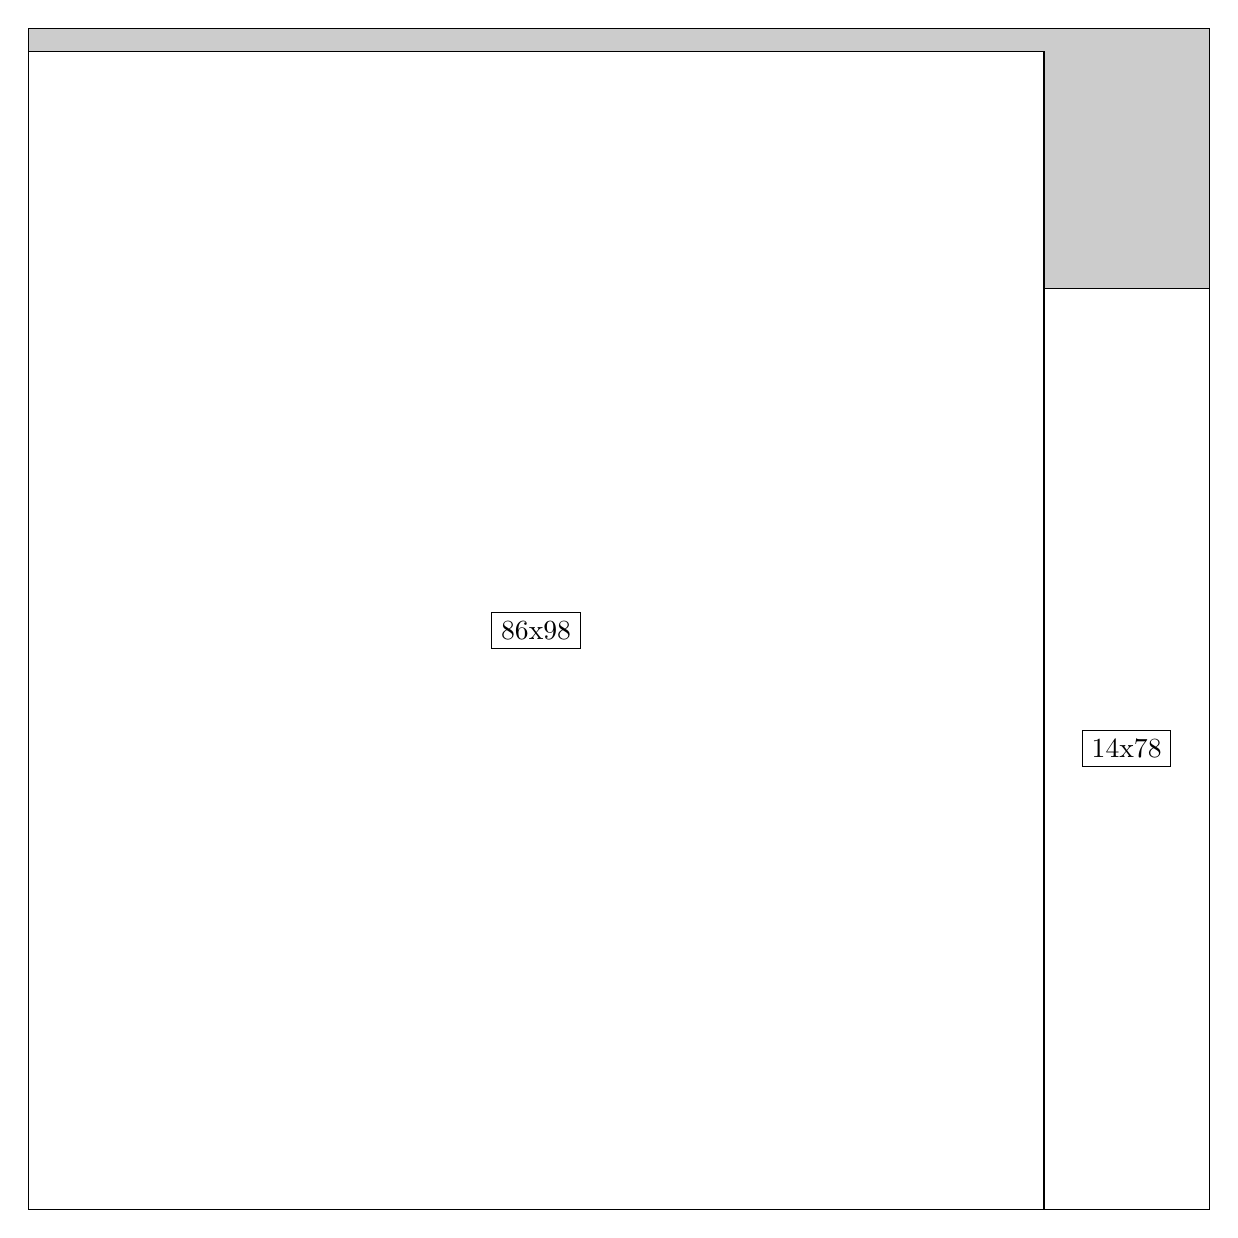
\begin{tikzpicture}[shorten >=1pt,scale=1.0,every node/.style={scale=1.0},->]
\tikzstyle{vertex}=[circle,fill=black!25,minimum size=14pt,inner sep=0pt]
\filldraw[fill=gray!40!white, draw=black] (0,0) rectangle (15.0,15.0);
\foreach \name/\x/\y/\w/\h in {86x98/0.0/0.0/12.9/14.7,14x78/12.9/0.0/2.1/11.7}
\filldraw[fill=white!40!white, draw=black] (\x,\y) rectangle node[draw] (\name) {\name} ++(\w,\h);
\end{tikzpicture}


w =86 , h =98 , x =0 , y =0 , v =8428
\par
w =14 , h =78 , x =86 , y =0 , v =1092
\par
\newpage


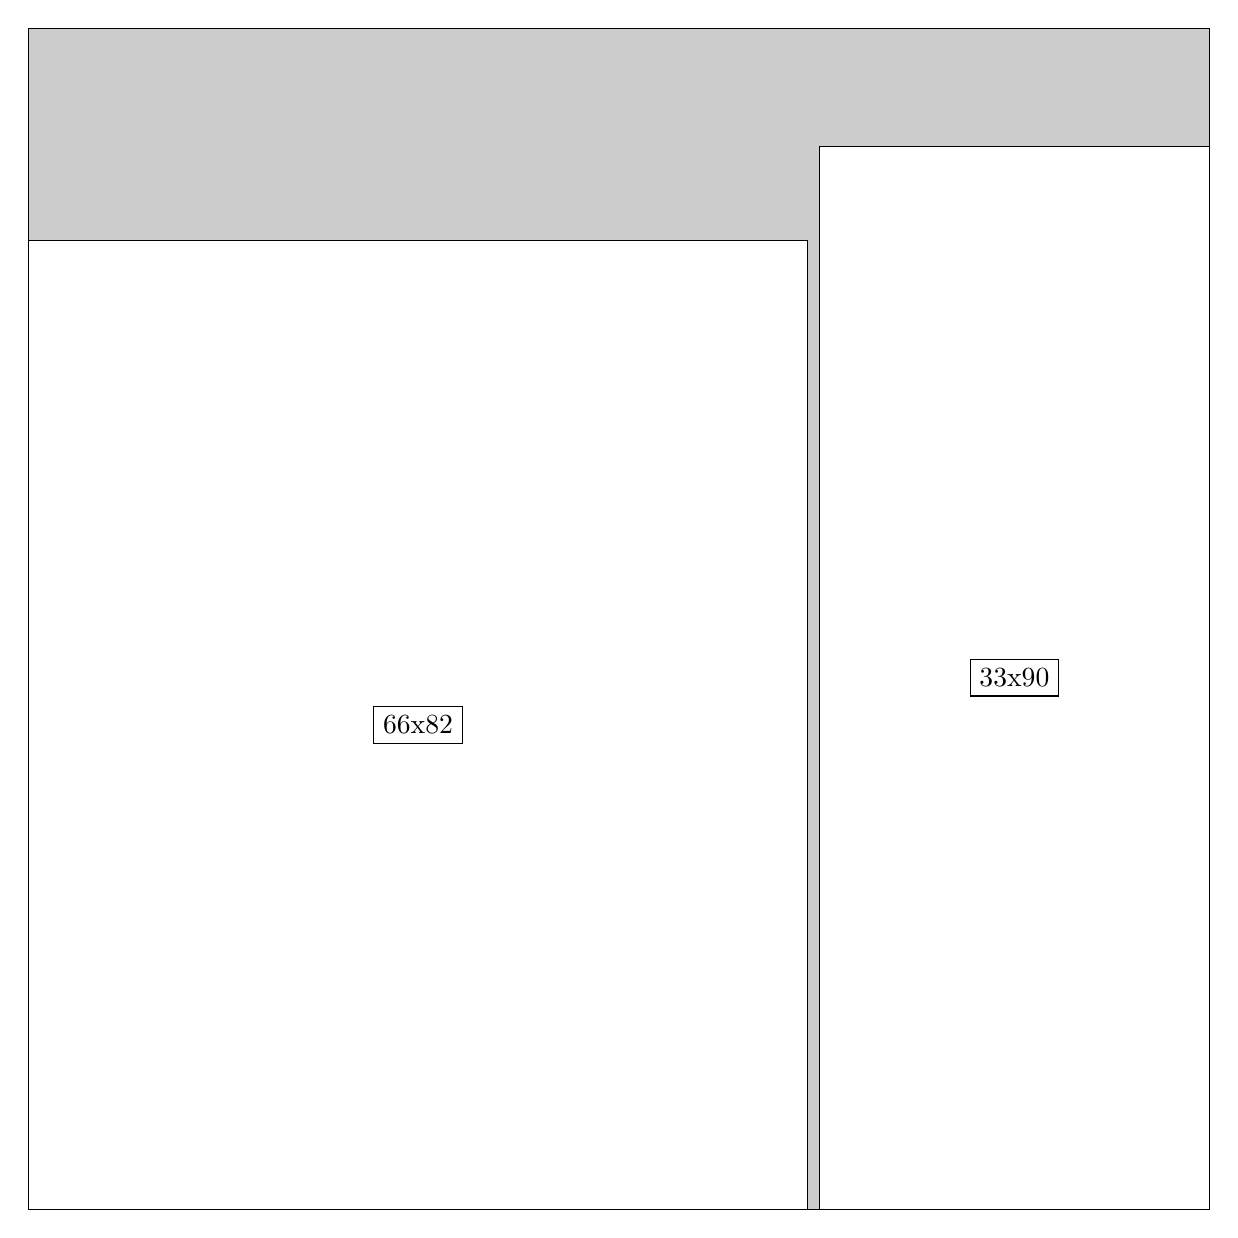
\begin{tikzpicture}[shorten >=1pt,scale=1.0,every node/.style={scale=1.0},->]
\tikzstyle{vertex}=[circle,fill=black!25,minimum size=14pt,inner sep=0pt]
\filldraw[fill=gray!40!white, draw=black] (0,0) rectangle (15.0,15.0);
\foreach \name/\x/\y/\w/\h in {66x82/0.0/0.0/9.9/12.299999999999999,33x90/10.049999999999999/0.0/4.95/13.5}
\filldraw[fill=white!40!white, draw=black] (\x,\y) rectangle node[draw] (\name) {\name} ++(\w,\h);
\end{tikzpicture}


w =66 , h =82 , x =0 , y =0 , v =5412
\par
w =33 , h =90 , x =67 , y =0 , v =2970
\par
\newpage


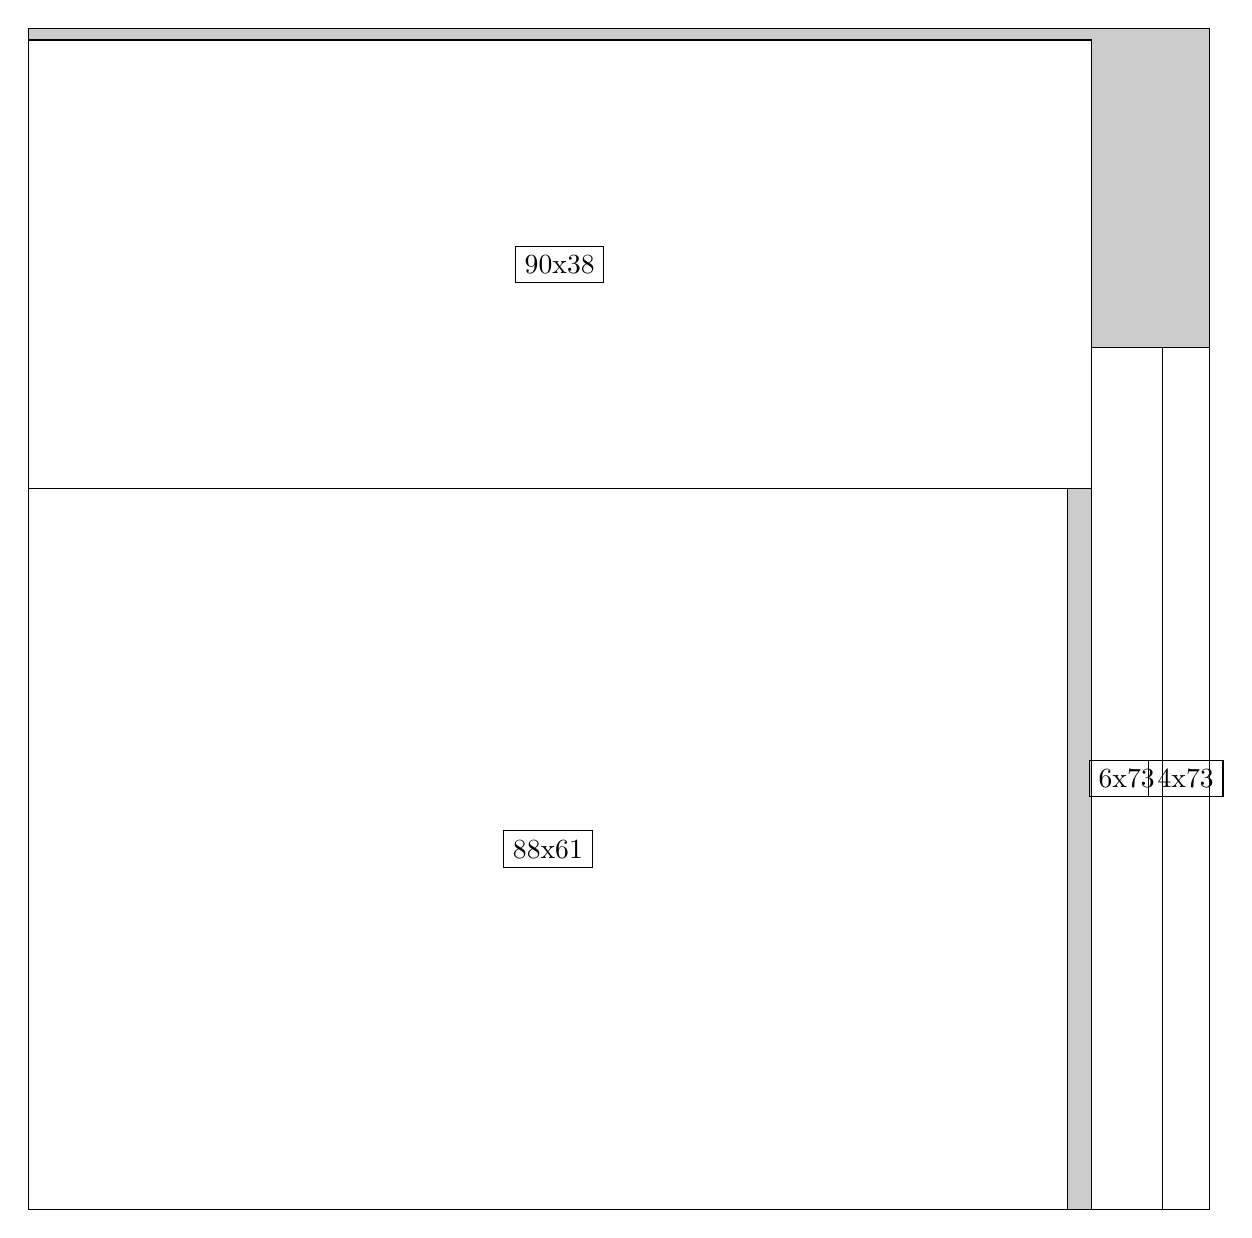
\begin{tikzpicture}[shorten >=1pt,scale=1.0,every node/.style={scale=1.0},->]
\tikzstyle{vertex}=[circle,fill=black!25,minimum size=14pt,inner sep=0pt]
\filldraw[fill=gray!40!white, draw=black] (0,0) rectangle (15.0,15.0);
\foreach \name/\x/\y/\w/\h in {88x61/0.0/0.0/13.2/9.15,90x38/0.0/9.15/13.5/5.7,6x73/13.5/0.0/0.8999999999999999/10.95,4x73/14.399999999999999/0.0/0.6/10.95}
\filldraw[fill=white!40!white, draw=black] (\x,\y) rectangle node[draw] (\name) {\name} ++(\w,\h);
\end{tikzpicture}


w =88 , h =61 , x =0 , y =0 , v =5368
\par
w =90 , h =38 , x =0 , y =61 , v =3420
\par
w =6 , h =73 , x =90 , y =0 , v =438
\par
w =4 , h =73 , x =96 , y =0 , v =292
\par
\newpage


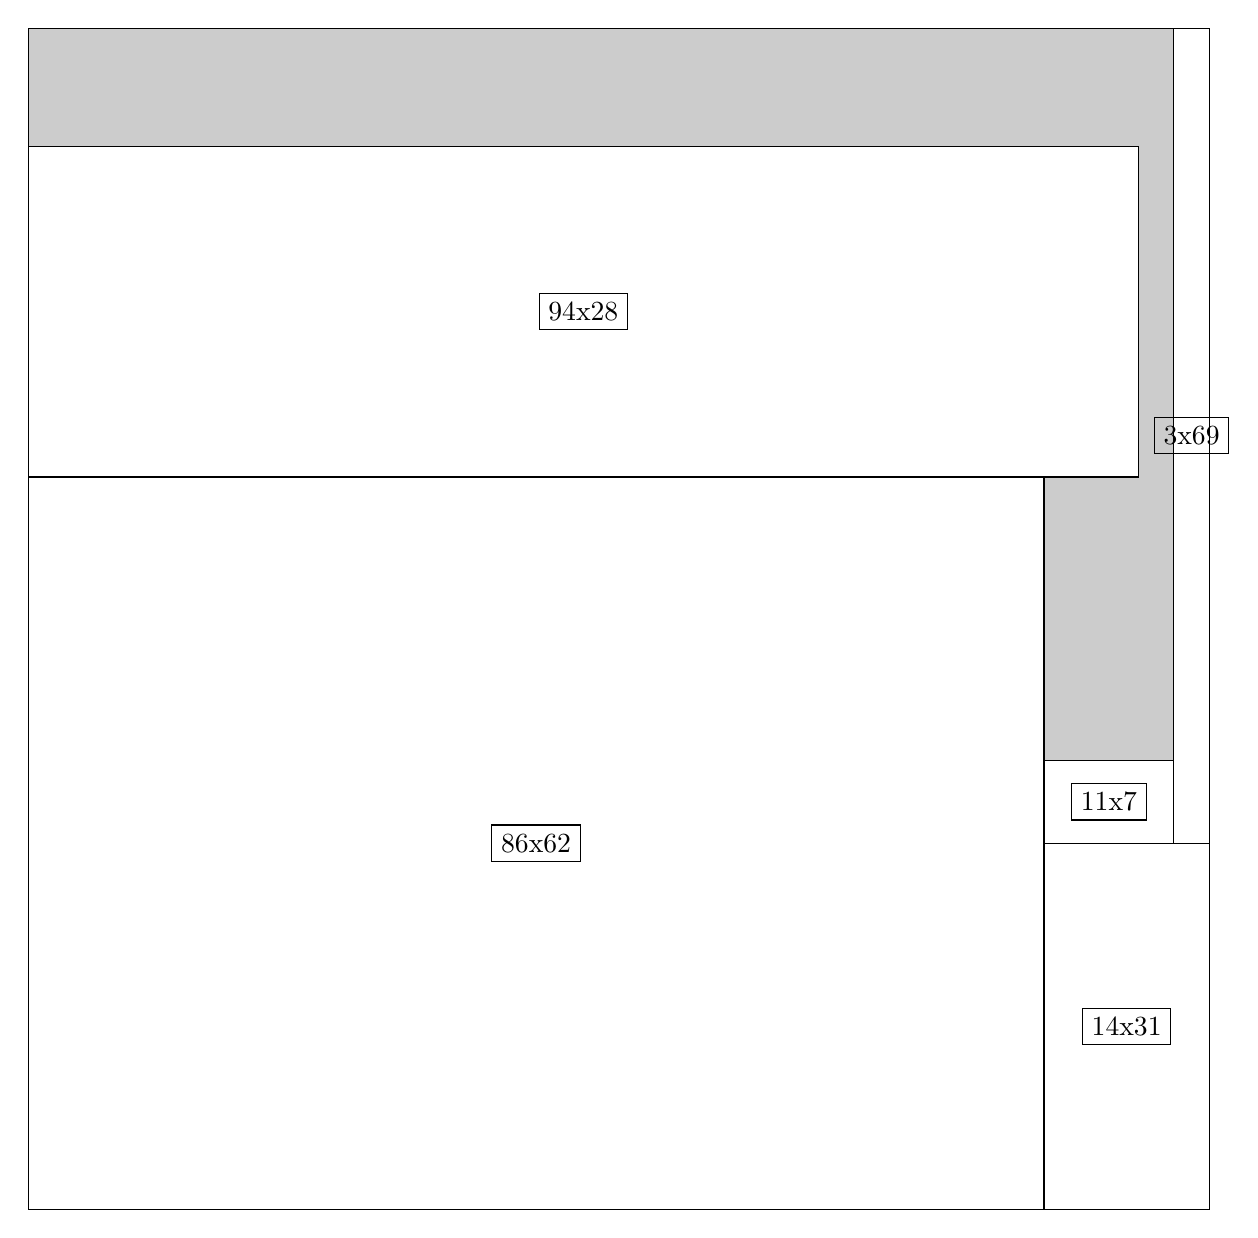
\begin{tikzpicture}[shorten >=1pt,scale=1.0,every node/.style={scale=1.0},->]
\tikzstyle{vertex}=[circle,fill=black!25,minimum size=14pt,inner sep=0pt]
\filldraw[fill=gray!40!white, draw=black] (0,0) rectangle (15.0,15.0);
\foreach \name/\x/\y/\w/\h in {86x62/0.0/0.0/12.9/9.299999999999999,94x28/0.0/9.299999999999999/14.1/4.2,14x31/12.9/0.0/2.1/4.6499999999999995,3x69/14.549999999999999/4.6499999999999995/0.44999999999999996/10.35,11x7/12.9/4.6499999999999995/1.65/1.05}
\filldraw[fill=white!40!white, draw=black] (\x,\y) rectangle node[draw] (\name) {\name} ++(\w,\h);
\end{tikzpicture}


w =86 , h =62 , x =0 , y =0 , v =5332
\par
w =94 , h =28 , x =0 , y =62 , v =2632
\par
w =14 , h =31 , x =86 , y =0 , v =434
\par
w =3 , h =69 , x =97 , y =31 , v =207
\par
w =11 , h =7 , x =86 , y =31 , v =77
\par
\newpage


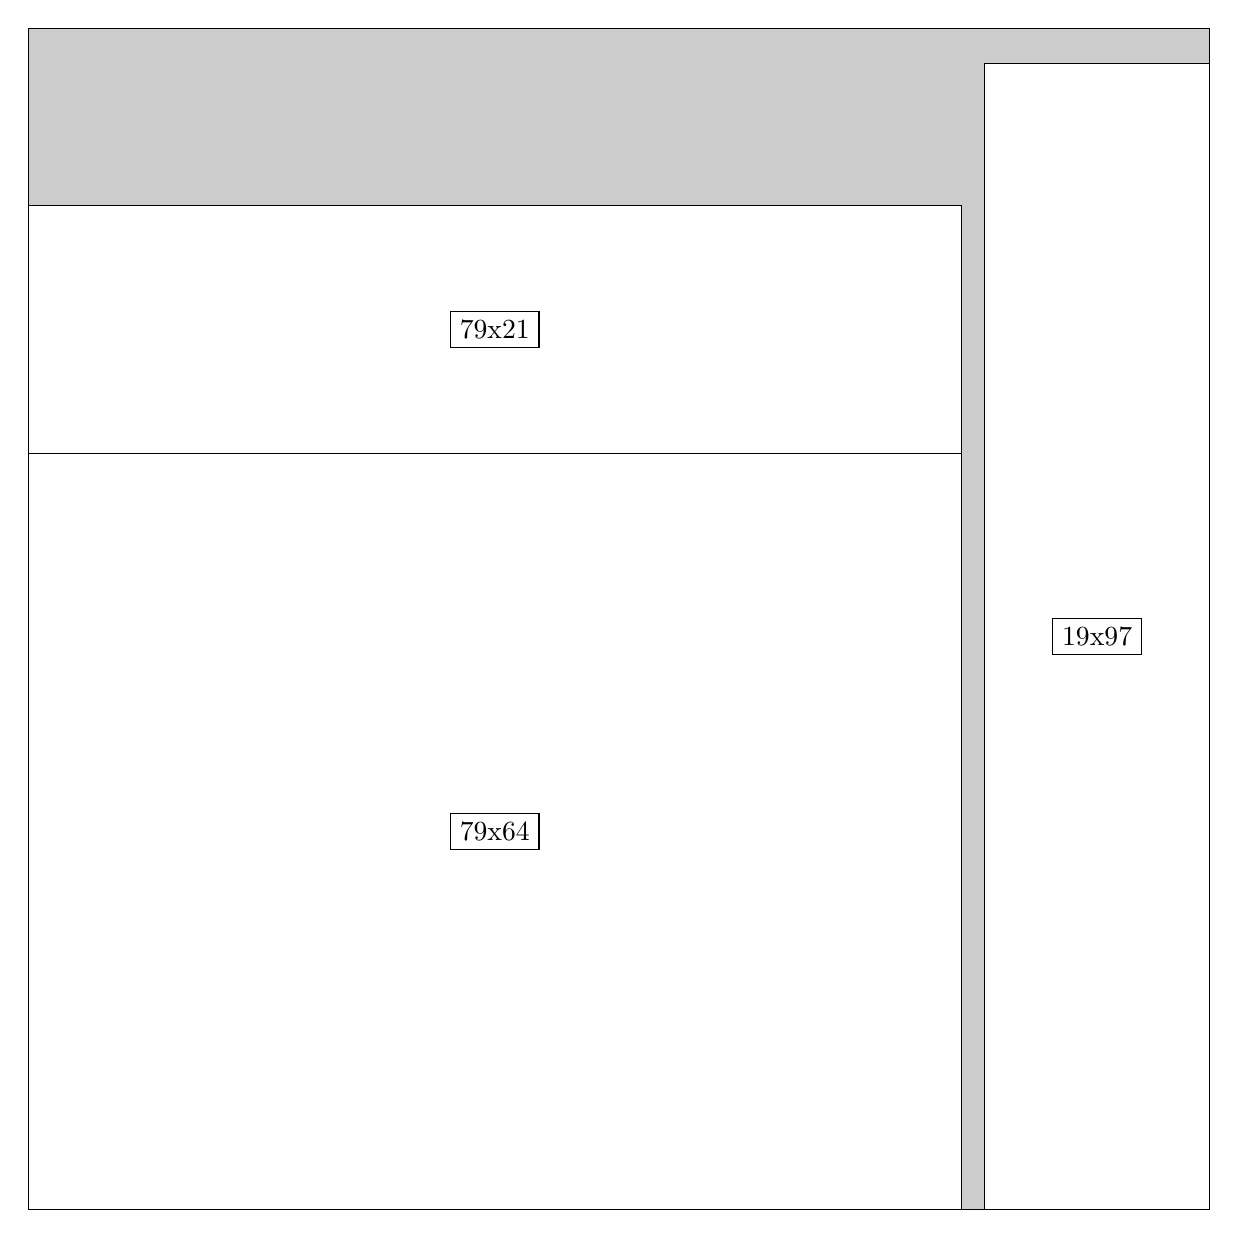
\begin{tikzpicture}[shorten >=1pt,scale=1.0,every node/.style={scale=1.0},->]
\tikzstyle{vertex}=[circle,fill=black!25,minimum size=14pt,inner sep=0pt]
\filldraw[fill=gray!40!white, draw=black] (0,0) rectangle (15.0,15.0);
\foreach \name/\x/\y/\w/\h in {79x64/0.0/0.0/11.85/9.6,19x97/12.15/0.0/2.85/14.549999999999999,79x21/0.0/9.6/11.85/3.15}
\filldraw[fill=white!40!white, draw=black] (\x,\y) rectangle node[draw] (\name) {\name} ++(\w,\h);
\end{tikzpicture}


w =79 , h =64 , x =0 , y =0 , v =5056
\par
w =19 , h =97 , x =81 , y =0 , v =1843
\par
w =79 , h =21 , x =0 , y =64 , v =1659
\par
\newpage


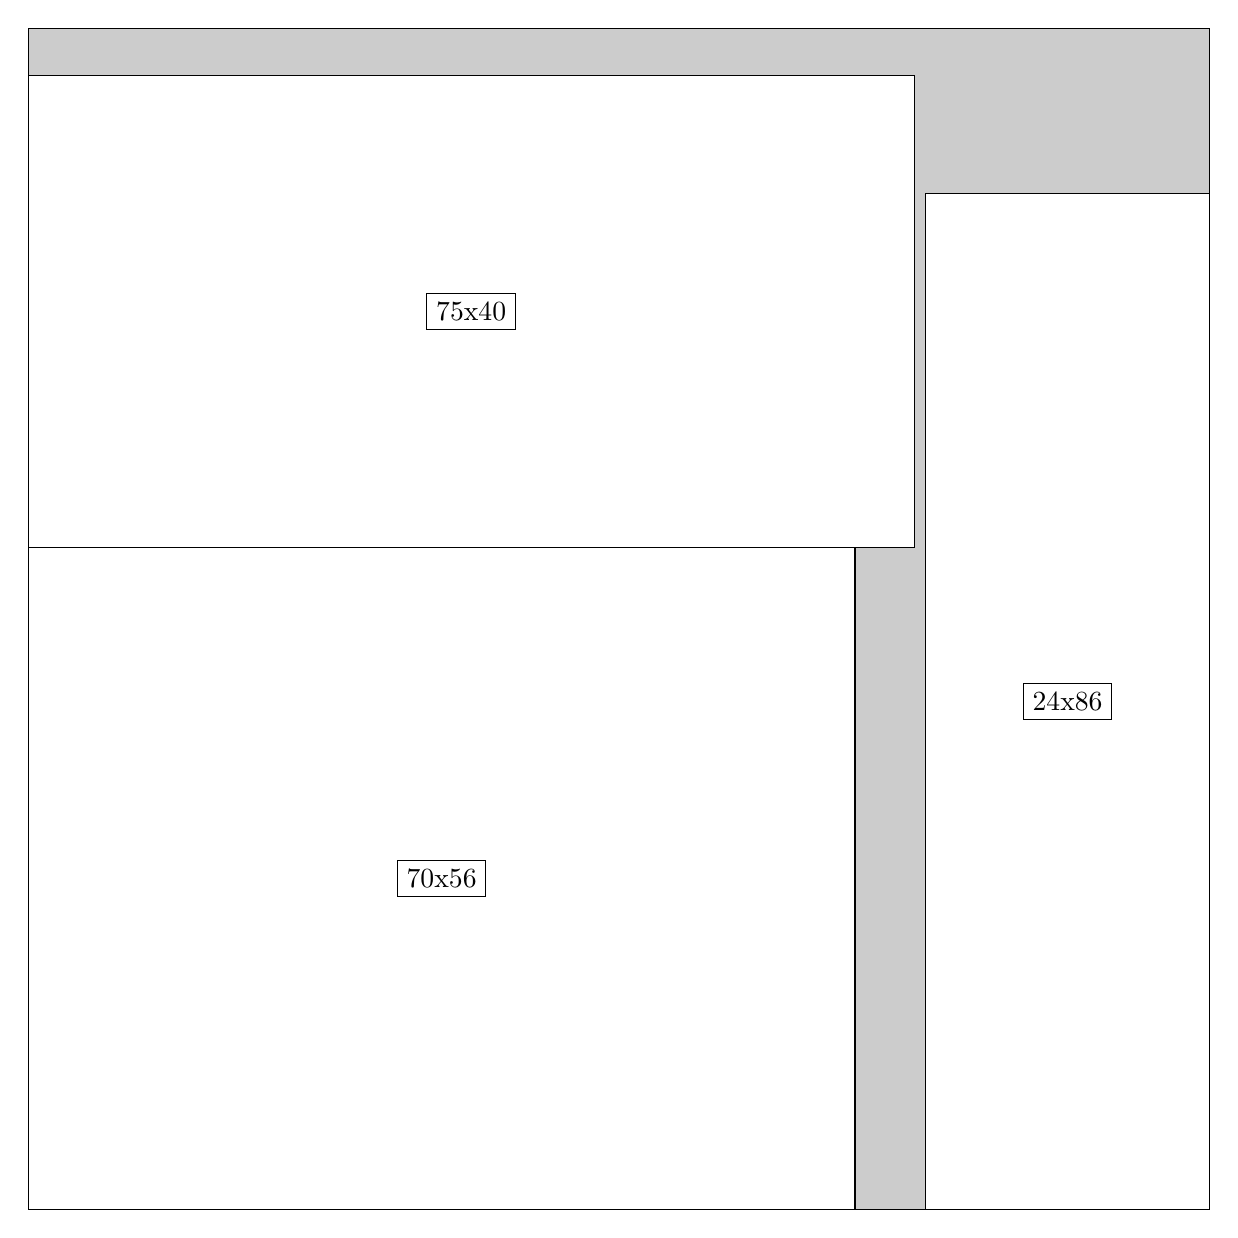
\begin{tikzpicture}[shorten >=1pt,scale=1.0,every node/.style={scale=1.0},->]
\tikzstyle{vertex}=[circle,fill=black!25,minimum size=14pt,inner sep=0pt]
\filldraw[fill=gray!40!white, draw=black] (0,0) rectangle (15.0,15.0);
\foreach \name/\x/\y/\w/\h in {70x56/0.0/0.0/10.5/8.4,75x40/0.0/8.4/11.25/6.0,24x86/11.4/0.0/3.5999999999999996/12.9}
\filldraw[fill=white!40!white, draw=black] (\x,\y) rectangle node[draw] (\name) {\name} ++(\w,\h);
\end{tikzpicture}


w =70 , h =56 , x =0 , y =0 , v =3920
\par
w =75 , h =40 , x =0 , y =56 , v =3000
\par
w =24 , h =86 , x =76 , y =0 , v =2064
\par
\newpage


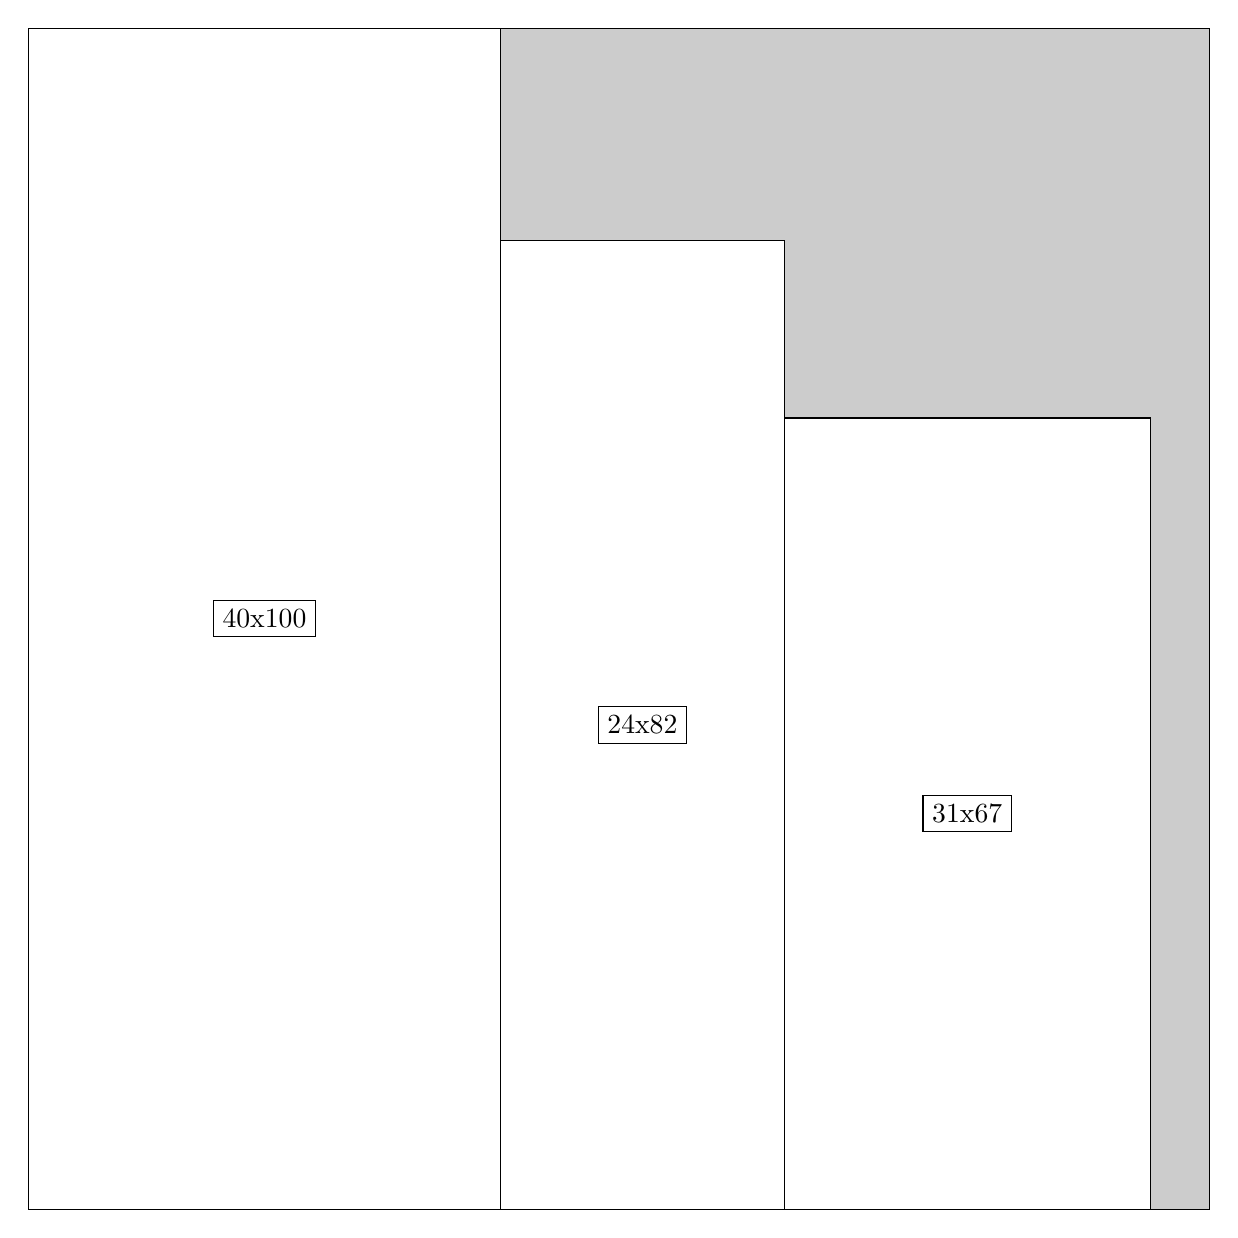
\begin{tikzpicture}[shorten >=1pt,scale=1.0,every node/.style={scale=1.0},->]
\tikzstyle{vertex}=[circle,fill=black!25,minimum size=14pt,inner sep=0pt]
\filldraw[fill=gray!40!white, draw=black] (0,0) rectangle (15.0,15.0);
\foreach \name/\x/\y/\w/\h in {40x100/0.0/0.0/6.0/15.0,31x67/9.6/0.0/4.6499999999999995/10.049999999999999,24x82/6.0/0.0/3.5999999999999996/12.299999999999999}
\filldraw[fill=white!40!white, draw=black] (\x,\y) rectangle node[draw] (\name) {\name} ++(\w,\h);
\end{tikzpicture}


w =40 , h =100 , x =0 , y =0 , v =4000
\par
w =31 , h =67 , x =64 , y =0 , v =2077
\par
w =24 , h =82 , x =40 , y =0 , v =1968
\par
\newpage


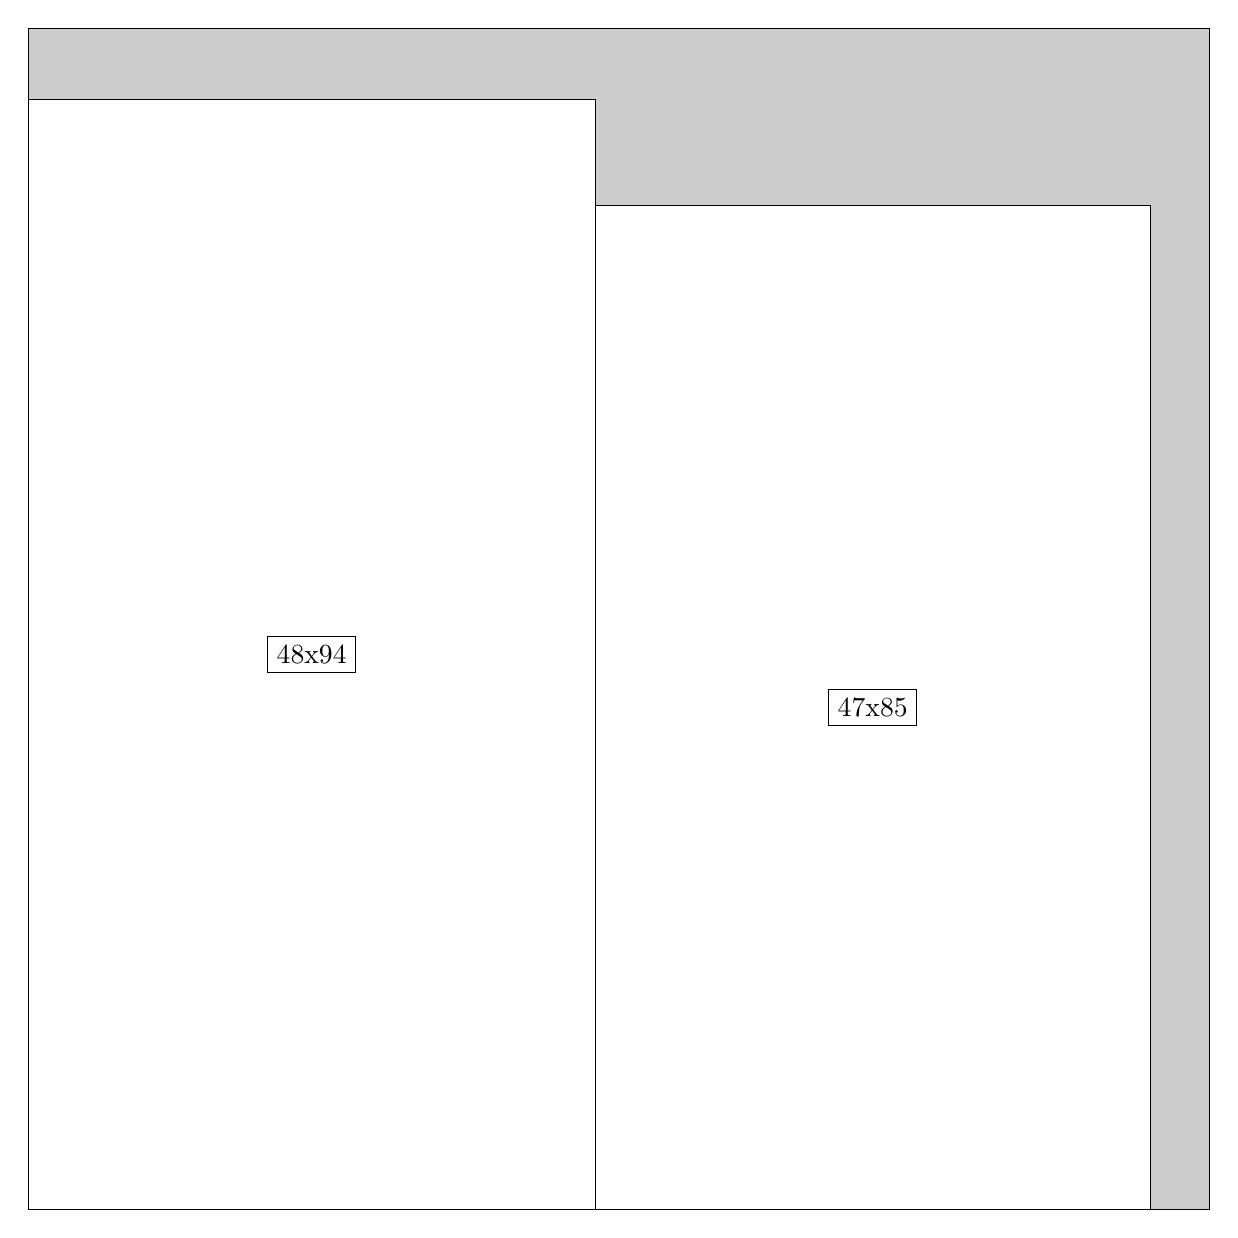
\begin{tikzpicture}[shorten >=1pt,scale=1.0,every node/.style={scale=1.0},->]
\tikzstyle{vertex}=[circle,fill=black!25,minimum size=14pt,inner sep=0pt]
\filldraw[fill=gray!40!white, draw=black] (0,0) rectangle (15.0,15.0);
\foreach \name/\x/\y/\w/\h in {48x94/0.0/0.0/7.199999999999999/14.1,47x85/7.199999999999999/0.0/7.05/12.75}
\filldraw[fill=white!40!white, draw=black] (\x,\y) rectangle node[draw] (\name) {\name} ++(\w,\h);
\end{tikzpicture}


w =48 , h =94 , x =0 , y =0 , v =4512
\par
w =47 , h =85 , x =48 , y =0 , v =3995
\par
\newpage


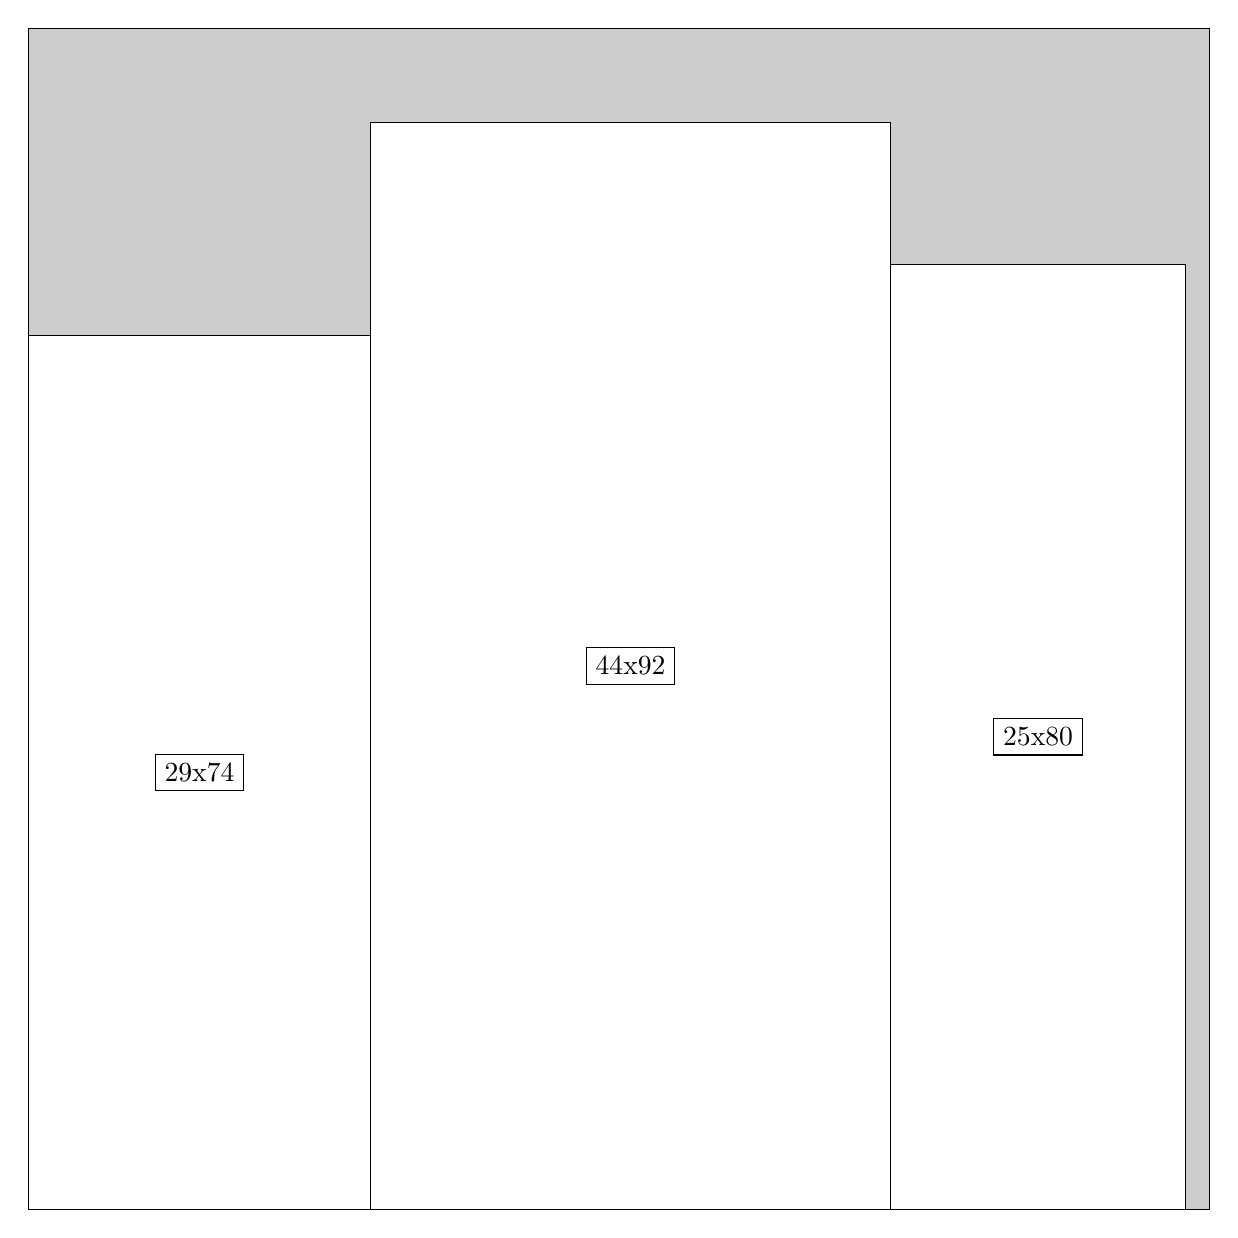
\begin{tikzpicture}[shorten >=1pt,scale=1.0,every node/.style={scale=1.0},->]
\tikzstyle{vertex}=[circle,fill=black!25,minimum size=14pt,inner sep=0pt]
\filldraw[fill=gray!40!white, draw=black] (0,0) rectangle (15.0,15.0);
\foreach \name/\x/\y/\w/\h in {29x74/0.0/0.0/4.35/11.1,44x92/4.35/0.0/6.6/13.799999999999999,25x80/10.95/0.0/3.75/12.0}
\filldraw[fill=white!40!white, draw=black] (\x,\y) rectangle node[draw] (\name) {\name} ++(\w,\h);
\end{tikzpicture}


w =29 , h =74 , x =0 , y =0 , v =2146
\par
w =44 , h =92 , x =29 , y =0 , v =4048
\par
w =25 , h =80 , x =73 , y =0 , v =2000
\par
\newpage


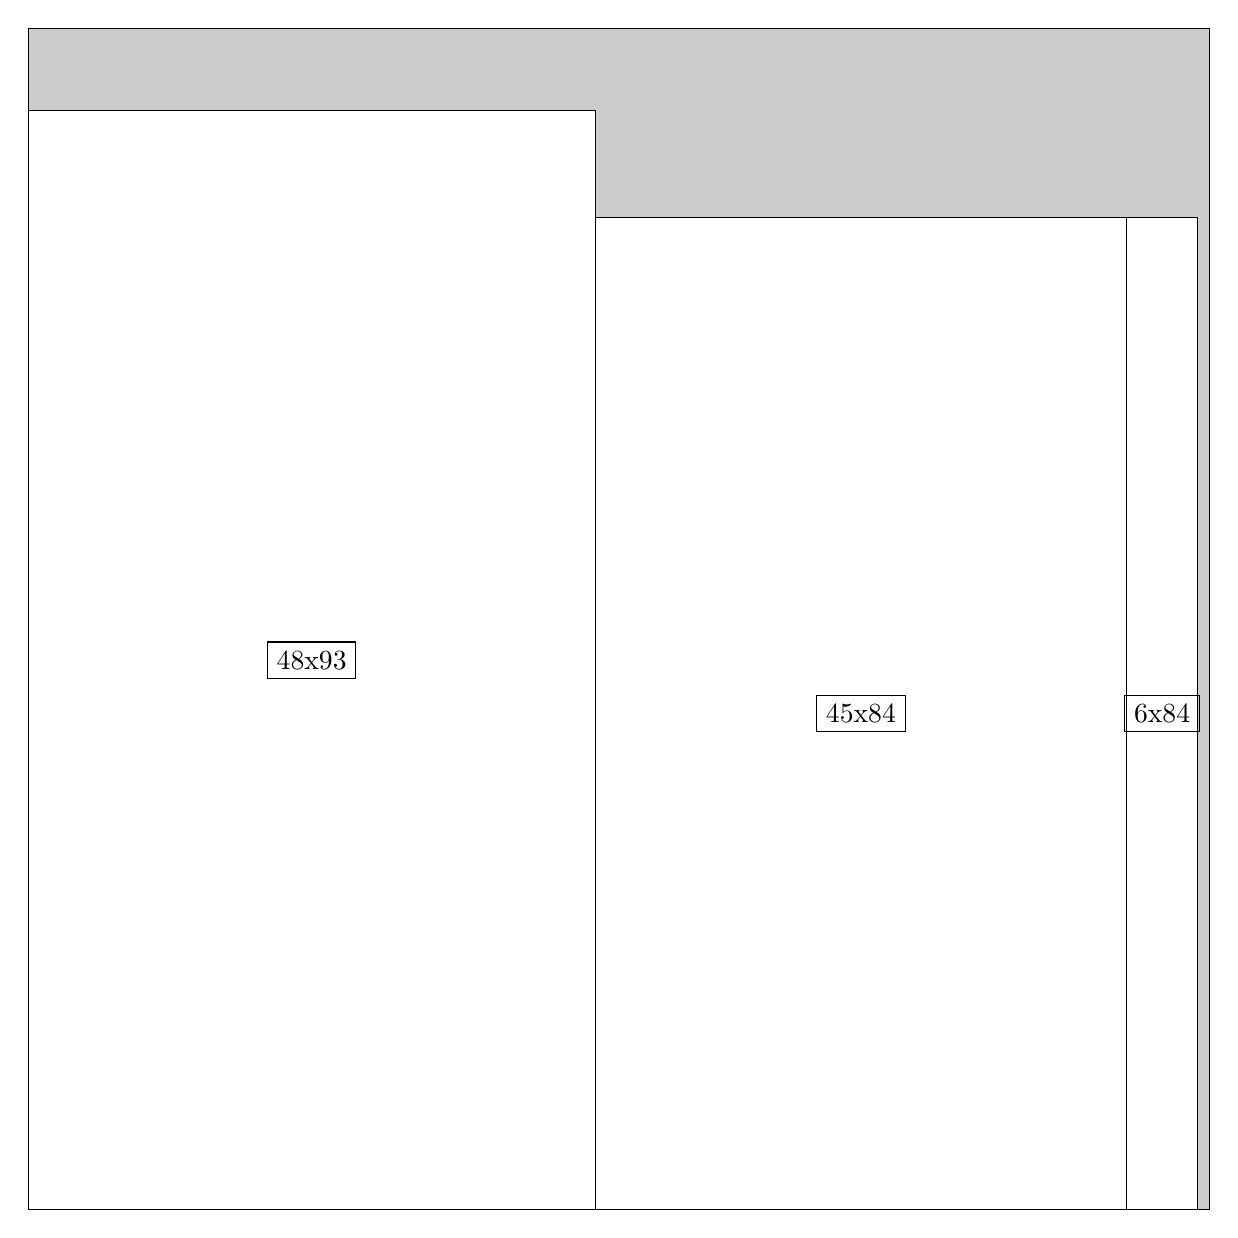
\begin{tikzpicture}[shorten >=1pt,scale=1.0,every node/.style={scale=1.0},->]
\tikzstyle{vertex}=[circle,fill=black!25,minimum size=14pt,inner sep=0pt]
\filldraw[fill=gray!40!white, draw=black] (0,0) rectangle (15.0,15.0);
\foreach \name/\x/\y/\w/\h in {48x93/0.0/0.0/7.199999999999999/13.95,45x84/7.199999999999999/0.0/6.75/12.6,6x84/13.95/0.0/0.8999999999999999/12.6}
\filldraw[fill=white!40!white, draw=black] (\x,\y) rectangle node[draw] (\name) {\name} ++(\w,\h);
\end{tikzpicture}


w =48 , h =93 , x =0 , y =0 , v =4464
\par
w =45 , h =84 , x =48 , y =0 , v =3780
\par
w =6 , h =84 , x =93 , y =0 , v =504
\par
\newpage


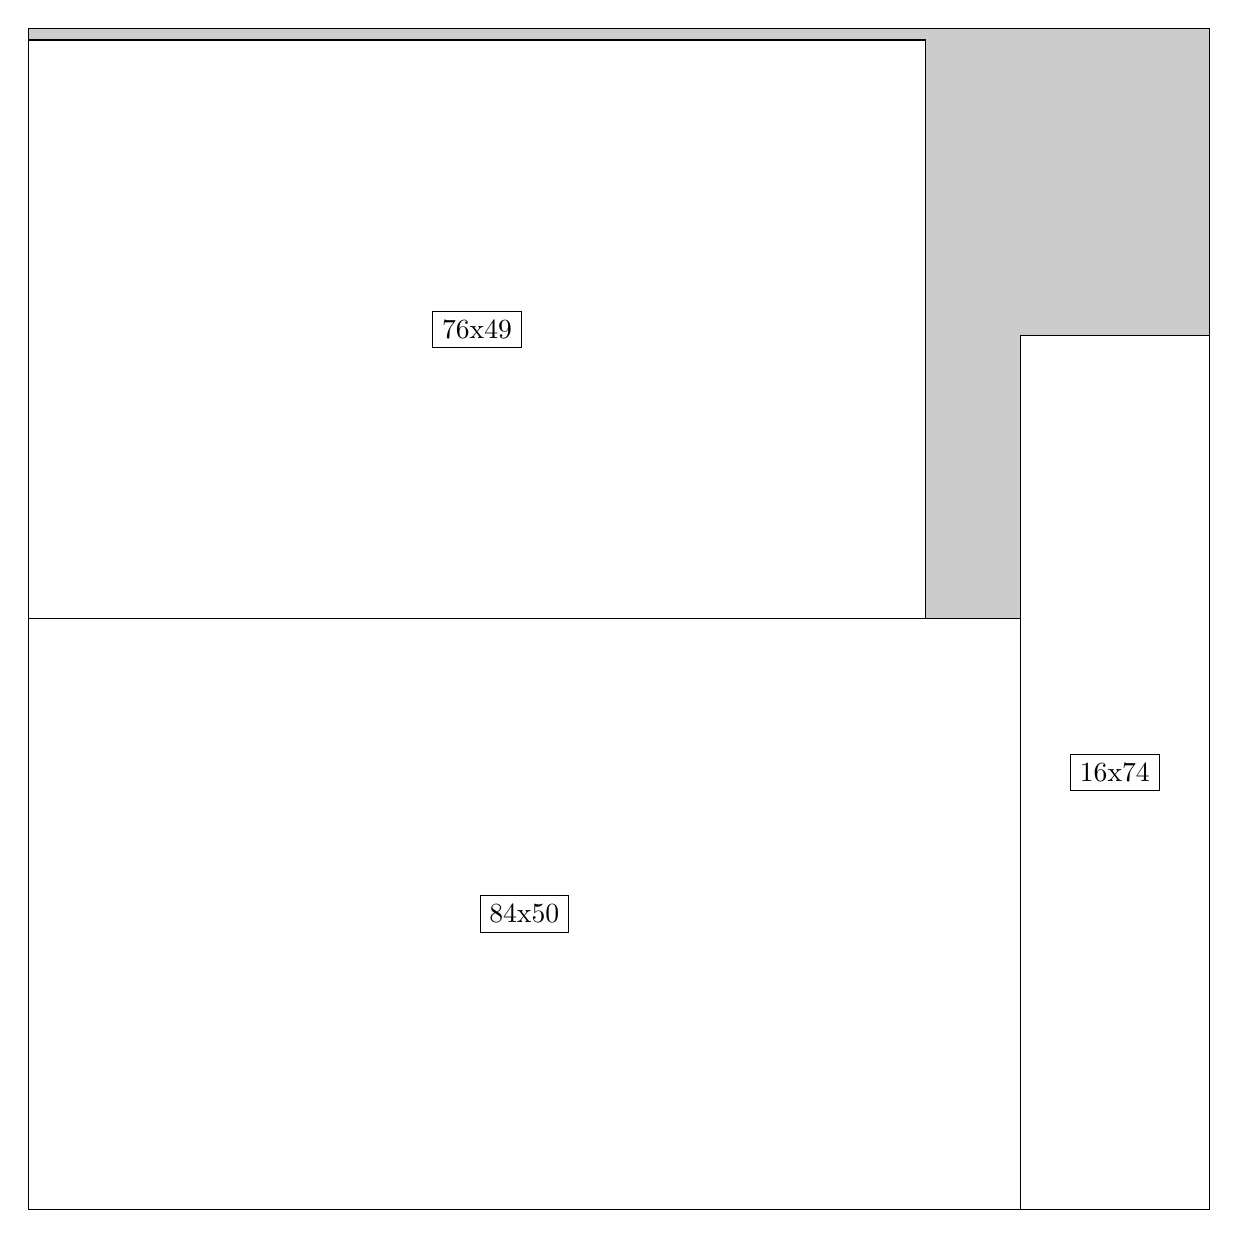
\begin{tikzpicture}[shorten >=1pt,scale=1.0,every node/.style={scale=1.0},->]
\tikzstyle{vertex}=[circle,fill=black!25,minimum size=14pt,inner sep=0pt]
\filldraw[fill=gray!40!white, draw=black] (0,0) rectangle (15.0,15.0);
\foreach \name/\x/\y/\w/\h in {84x50/0.0/0.0/12.6/7.5,76x49/0.0/7.5/11.4/7.35,16x74/12.6/0.0/2.4/11.1}
\filldraw[fill=white!40!white, draw=black] (\x,\y) rectangle node[draw] (\name) {\name} ++(\w,\h);
\end{tikzpicture}


w =84 , h =50 , x =0 , y =0 , v =4200
\par
w =76 , h =49 , x =0 , y =50 , v =3724
\par
w =16 , h =74 , x =84 , y =0 , v =1184
\par
\newpage


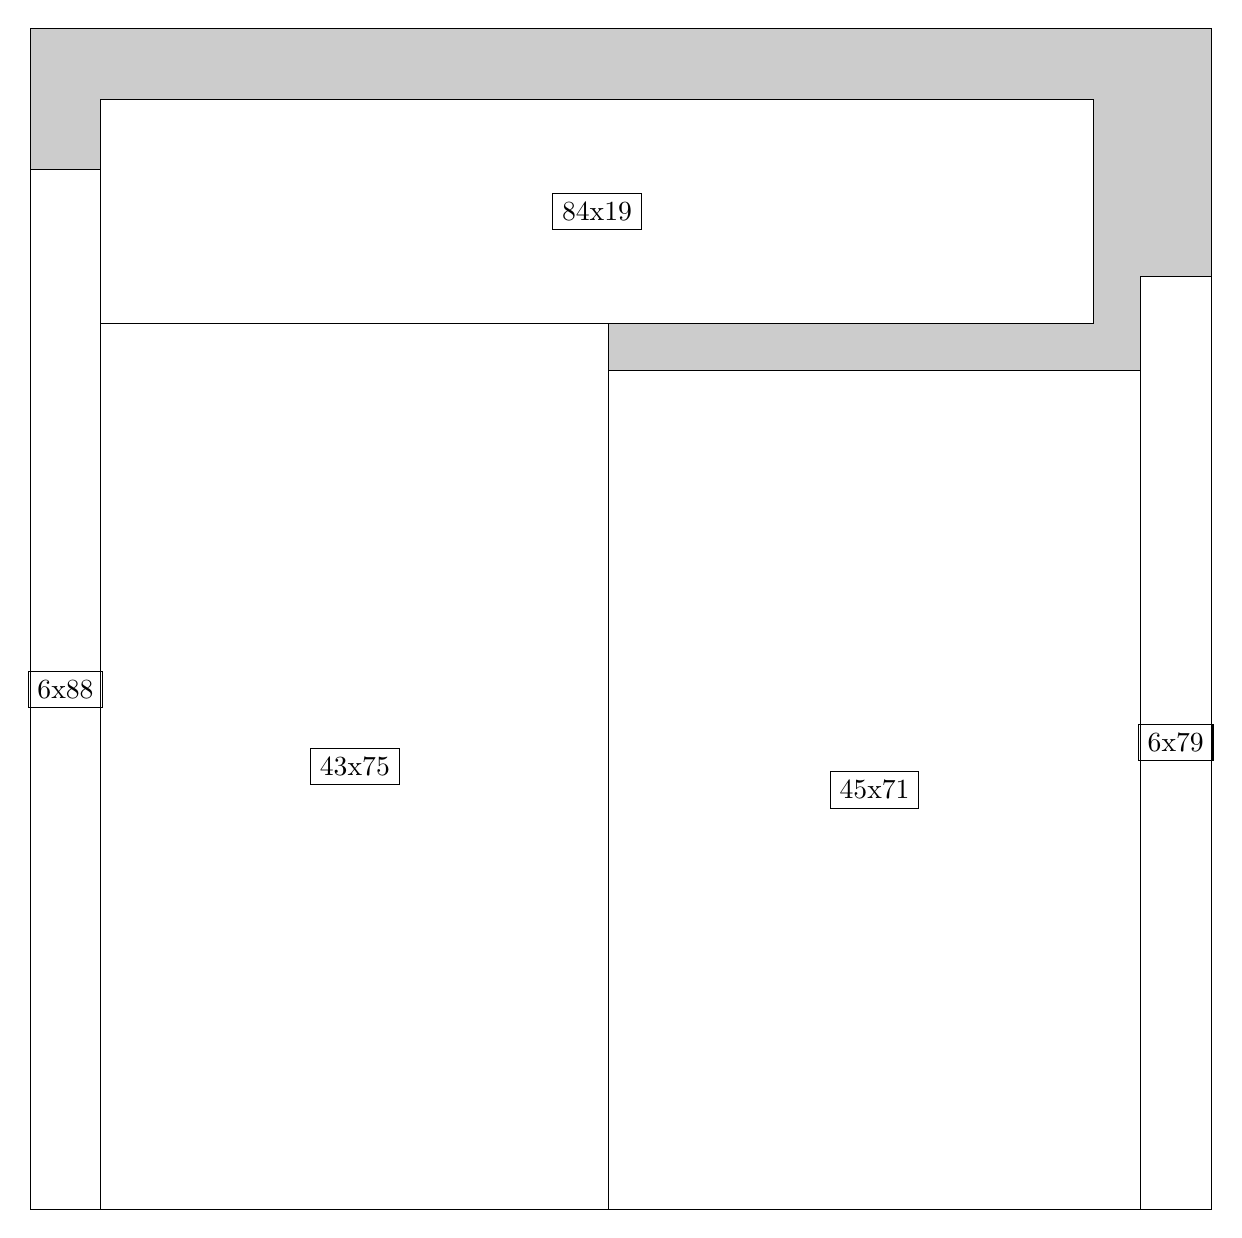
\begin{tikzpicture}[shorten >=1pt,scale=1.0,every node/.style={scale=1.0},->]
\tikzstyle{vertex}=[circle,fill=black!25,minimum size=14pt,inner sep=0pt]
\filldraw[fill=gray!40!white, draw=black] (0,0) rectangle (15.0,15.0);
\foreach \name/\x/\y/\w/\h in {43x75/0.8999999999999999/0.0/6.45/11.25,45x71/7.35/0.0/6.75/10.65,84x19/0.8999999999999999/11.25/12.6/2.85,6x88/0.0/0.0/0.8999999999999999/13.2,6x79/14.1/0.0/0.8999999999999999/11.85}
\filldraw[fill=white!40!white, draw=black] (\x,\y) rectangle node[draw] (\name) {\name} ++(\w,\h);
\end{tikzpicture}


w =43 , h =75 , x =6 , y =0 , v =3225
\par
w =45 , h =71 , x =49 , y =0 , v =3195
\par
w =84 , h =19 , x =6 , y =75 , v =1596
\par
w =6 , h =88 , x =0 , y =0 , v =528
\par
w =6 , h =79 , x =94 , y =0 , v =474
\par
\newpage


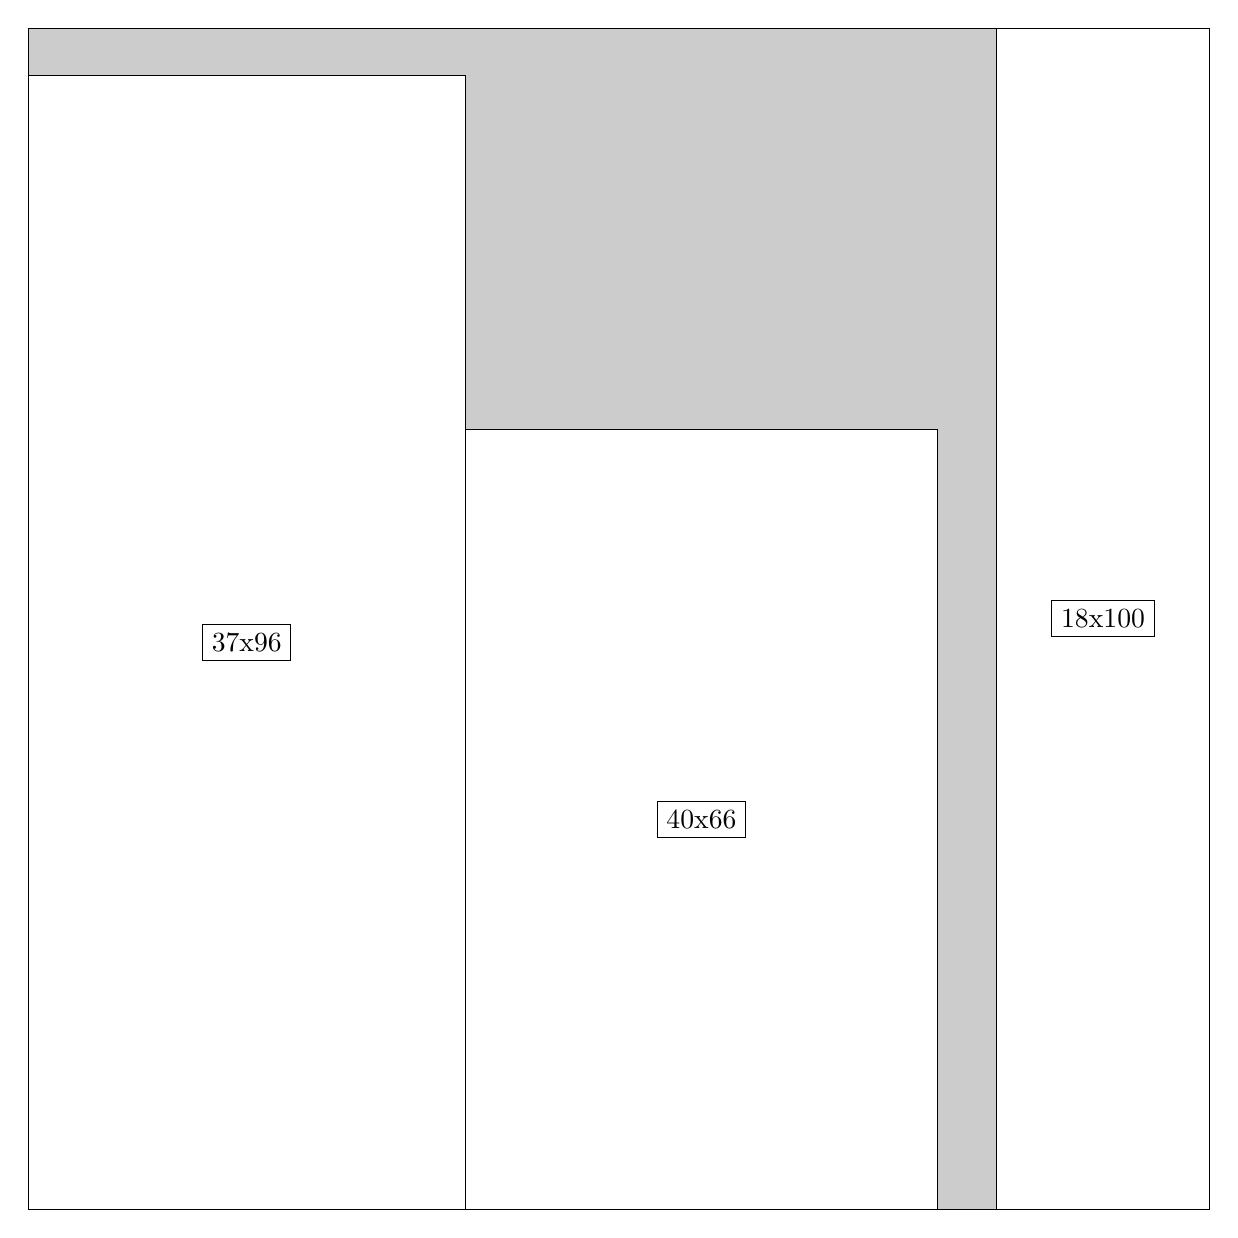
\begin{tikzpicture}[shorten >=1pt,scale=1.0,every node/.style={scale=1.0},->]
\tikzstyle{vertex}=[circle,fill=black!25,minimum size=14pt,inner sep=0pt]
\filldraw[fill=gray!40!white, draw=black] (0,0) rectangle (15.0,15.0);
\foreach \name/\x/\y/\w/\h in {37x96/0.0/0.0/5.55/14.399999999999999,40x66/5.55/0.0/6.0/9.9,18x100/12.299999999999999/0.0/2.6999999999999997/15.0}
\filldraw[fill=white!40!white, draw=black] (\x,\y) rectangle node[draw] (\name) {\name} ++(\w,\h);
\end{tikzpicture}


w =37 , h =96 , x =0 , y =0 , v =3552
\par
w =40 , h =66 , x =37 , y =0 , v =2640
\par
w =18 , h =100 , x =82 , y =0 , v =1800
\par
\newpage


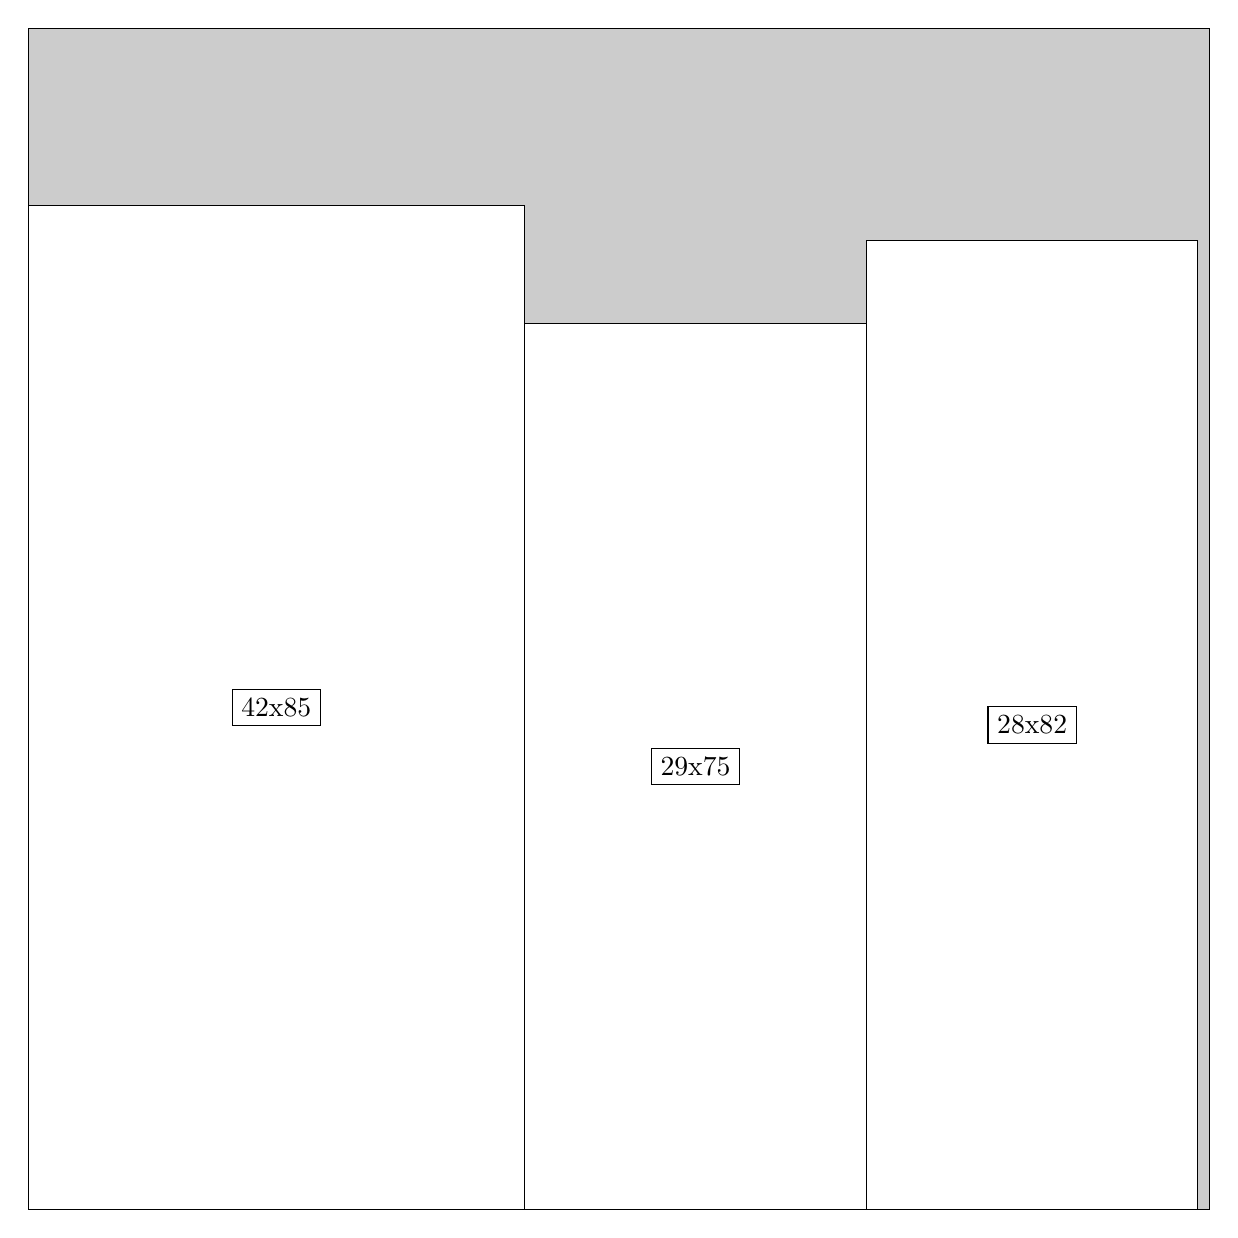
\begin{tikzpicture}[shorten >=1pt,scale=1.0,every node/.style={scale=1.0},->]
\tikzstyle{vertex}=[circle,fill=black!25,minimum size=14pt,inner sep=0pt]
\filldraw[fill=gray!40!white, draw=black] (0,0) rectangle (15.0,15.0);
\foreach \name/\x/\y/\w/\h in {42x85/0.0/0.0/6.3/12.75,29x75/6.3/0.0/4.35/11.25,28x82/10.65/0.0/4.2/12.299999999999999}
\filldraw[fill=white!40!white, draw=black] (\x,\y) rectangle node[draw] (\name) {\name} ++(\w,\h);
\end{tikzpicture}


w =42 , h =85 , x =0 , y =0 , v =3570
\par
w =29 , h =75 , x =42 , y =0 , v =2175
\par
w =28 , h =82 , x =71 , y =0 , v =2296
\par
\newpage


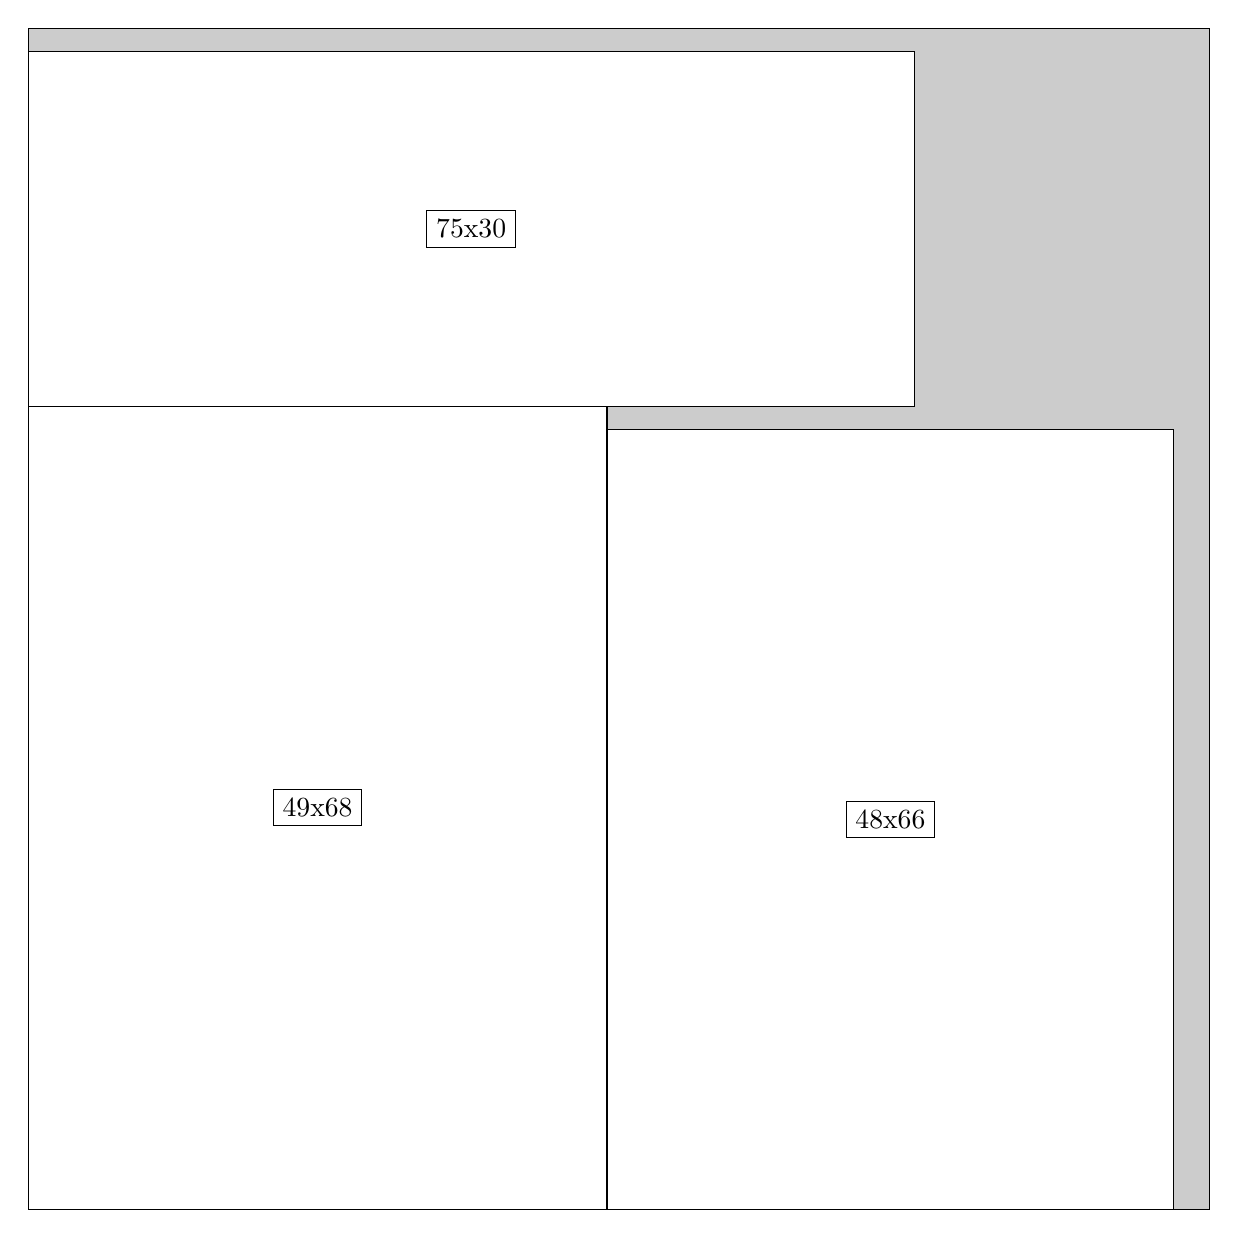
\begin{tikzpicture}[shorten >=1pt,scale=1.0,every node/.style={scale=1.0},->]
\tikzstyle{vertex}=[circle,fill=black!25,minimum size=14pt,inner sep=0pt]
\filldraw[fill=gray!40!white, draw=black] (0,0) rectangle (15.0,15.0);
\foreach \name/\x/\y/\w/\h in {49x68/0.0/0.0/7.35/10.2,48x66/7.35/0.0/7.199999999999999/9.9,75x30/0.0/10.2/11.25/4.5}
\filldraw[fill=white!40!white, draw=black] (\x,\y) rectangle node[draw] (\name) {\name} ++(\w,\h);
\end{tikzpicture}


w =49 , h =68 , x =0 , y =0 , v =3332
\par
w =48 , h =66 , x =49 , y =0 , v =3168
\par
w =75 , h =30 , x =0 , y =68 , v =2250
\par
\newpage


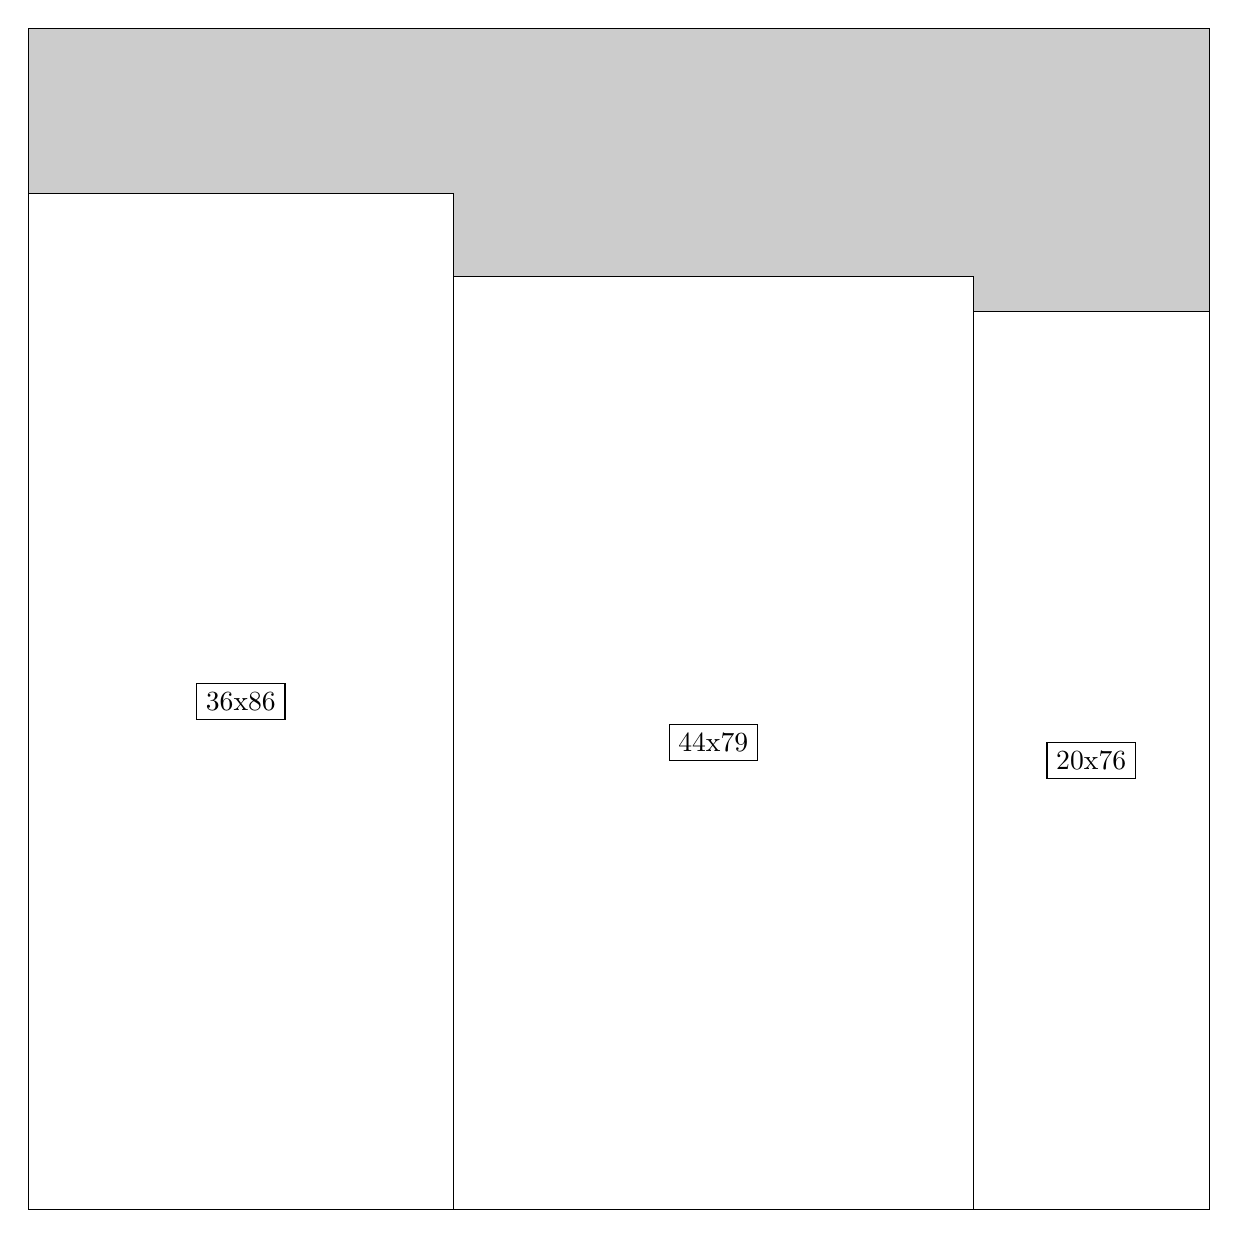
\begin{tikzpicture}[shorten >=1pt,scale=1.0,every node/.style={scale=1.0},->]
\tikzstyle{vertex}=[circle,fill=black!25,minimum size=14pt,inner sep=0pt]
\filldraw[fill=gray!40!white, draw=black] (0,0) rectangle (15.0,15.0);
\foreach \name/\x/\y/\w/\h in {44x79/5.3999999999999995/0.0/6.6/11.85,36x86/0.0/0.0/5.3999999999999995/12.9,20x76/12.0/0.0/3.0/11.4}
\filldraw[fill=white!40!white, draw=black] (\x,\y) rectangle node[draw] (\name) {\name} ++(\w,\h);
\end{tikzpicture}


w =44 , h =79 , x =36 , y =0 , v =3476
\par
w =36 , h =86 , x =0 , y =0 , v =3096
\par
w =20 , h =76 , x =80 , y =0 , v =1520
\par
\newpage


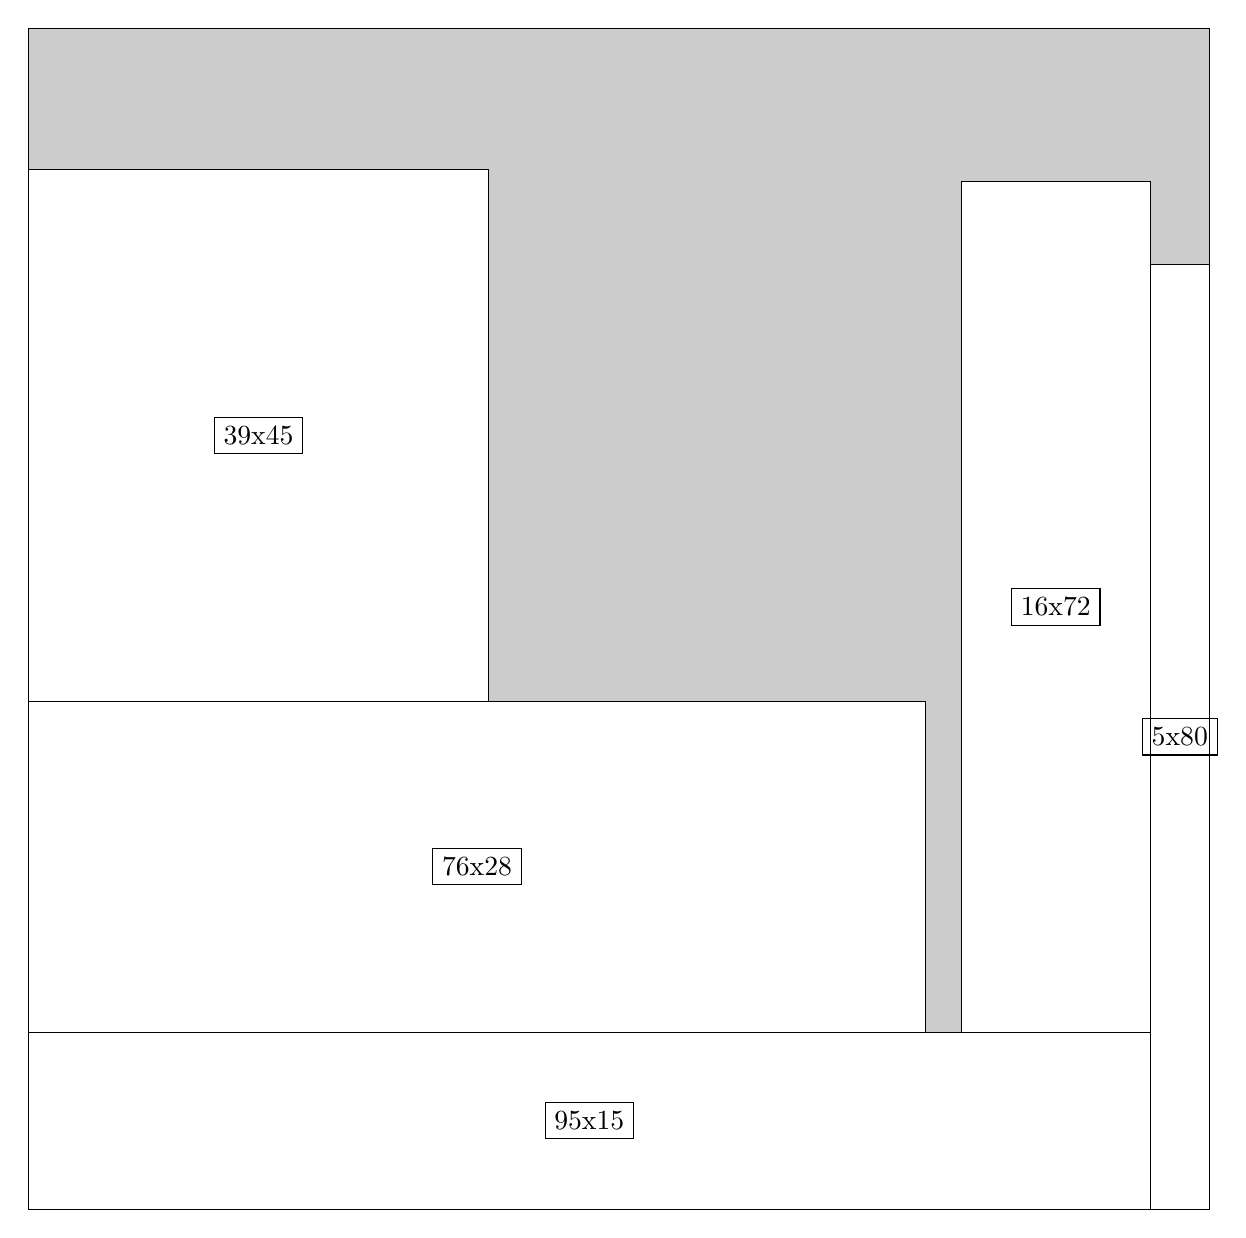
\begin{tikzpicture}[shorten >=1pt,scale=1.0,every node/.style={scale=1.0},->]
\tikzstyle{vertex}=[circle,fill=black!25,minimum size=14pt,inner sep=0pt]
\filldraw[fill=gray!40!white, draw=black] (0,0) rectangle (15.0,15.0);
\foreach \name/\x/\y/\w/\h in {95x15/0.0/0.0/14.25/2.25,76x28/0.0/2.25/11.4/4.2,39x45/0.0/6.45/5.85/6.75,16x72/11.85/2.25/2.4/10.799999999999999,5x80/14.25/0.0/0.75/12.0}
\filldraw[fill=white!40!white, draw=black] (\x,\y) rectangle node[draw] (\name) {\name} ++(\w,\h);
\end{tikzpicture}


w =95 , h =15 , x =0 , y =0 , v =1425
\par
w =76 , h =28 , x =0 , y =15 , v =2128
\par
w =39 , h =45 , x =0 , y =43 , v =1755
\par
w =16 , h =72 , x =79 , y =15 , v =1152
\par
w =5 , h =80 , x =95 , y =0 , v =400
\par
\newpage


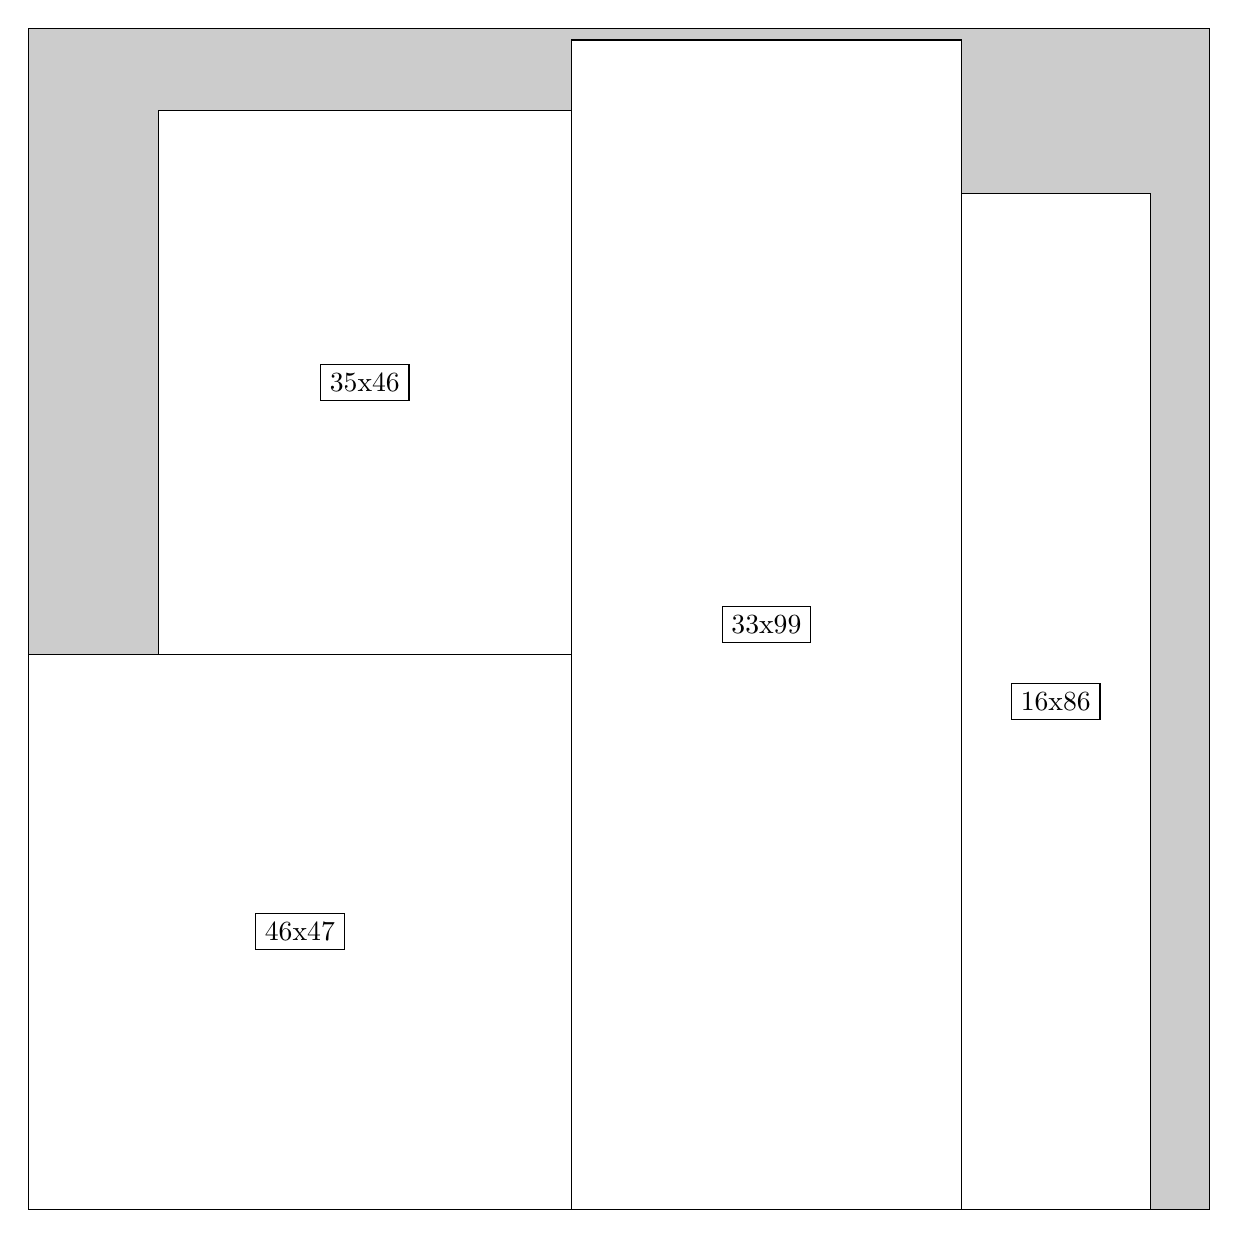
\begin{tikzpicture}[shorten >=1pt,scale=1.0,every node/.style={scale=1.0},->]
\tikzstyle{vertex}=[circle,fill=black!25,minimum size=14pt,inner sep=0pt]
\filldraw[fill=gray!40!white, draw=black] (0,0) rectangle (15.0,15.0);
\foreach \name/\x/\y/\w/\h in {33x99/6.8999999999999995/0.0/4.95/14.85,46x47/0.0/0.0/6.8999999999999995/7.05,35x46/1.65/7.05/5.25/6.8999999999999995,16x86/11.85/0.0/2.4/12.9}
\filldraw[fill=white!40!white, draw=black] (\x,\y) rectangle node[draw] (\name) {\name} ++(\w,\h);
\end{tikzpicture}


w =33 , h =99 , x =46 , y =0 , v =3267
\par
w =46 , h =47 , x =0 , y =0 , v =2162
\par
w =35 , h =46 , x =11 , y =47 , v =1610
\par
w =16 , h =86 , x =79 , y =0 , v =1376
\par
\newpage


\end{document}